


In this chapter I study the three methods for approximating the Langevin likelihood presented in chapter~\ref{chap: methods} by using simulations of the Langevin process. Throughout this chapter I will be simulating from the Langevin using the Euler-Maruyama method with the perlin noise Covariates presented in figure~\ref{fig:covariate plots} and a time resolution of $\Delta_t =0.01$.




\section{Using the Extended Kalman Filter}


to study the 
To test the likelihood approximation using the Extended Kalman filter, 100 tracks were simulated each with 5000 observations with a resolution of $\Delta t = 0.1$. For each track, the parameters $\gamma^2$ and $\beta$ were estimated using both the EKF likelihood and the estimator described in section~\ref{sec: estimating parameters}. The number of steps used in the extended Kalman filter was 10. From these estimates box-plots were made comparing the two methods for each of the parameters. The code used to implement this experiment can be found in the git hub repository in appendix~\ref{Appendix: github repo}. the results are shown in figure~\ref{fig:EKF_thin_boxplot}.

 

\begin{figure}[H]
    \centering
    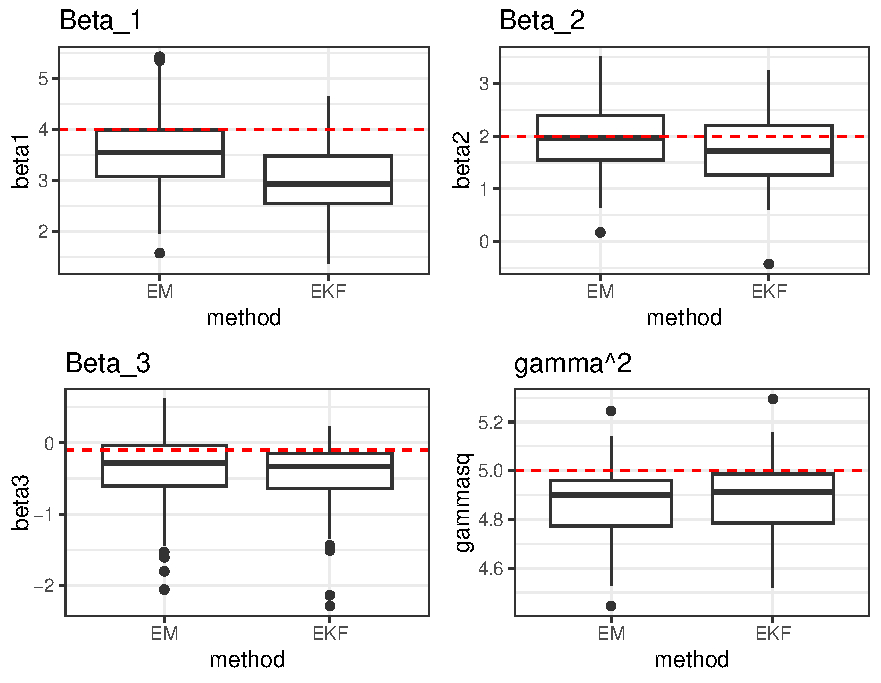
\includegraphics[width=\linewidth]{Images/Results/EM VS EKF boxplots.pdf}
    \caption[example 1 covariates]{Boxplots of estimated parameters for tracks with 1000 observation using the Euler-Maruyama method to the left and the extended Kalman filter to the right. The red line indicates the true value of the parameter.}
    \label{fig:EKF_thin_boxplot}
\end{figure}

Figure~\ref{fig:EM_thin_boxplot} shows that there is little or no improvement in the estimates from using the extended Kalman filter. for the $\beta$ parameters, then mean estimated parameter is further from the true value of the parameter than the mean of the estimates using the Euler-Maruyama method. For the estimates of $\gamma^2$ however, the mean of the estimates using the extended Kalman filter is slightly closer to the true value of the parameter than the mean of the estimates using the Euler Maruyama method. Overall there is an observable bias in the estimates using both these methods in all of the parameters.

\section{Brownian Bridge Importance Sampling Likelihood}

\subsection{Varying Time Resolution}


\begin{figure}[H]
    \centering
    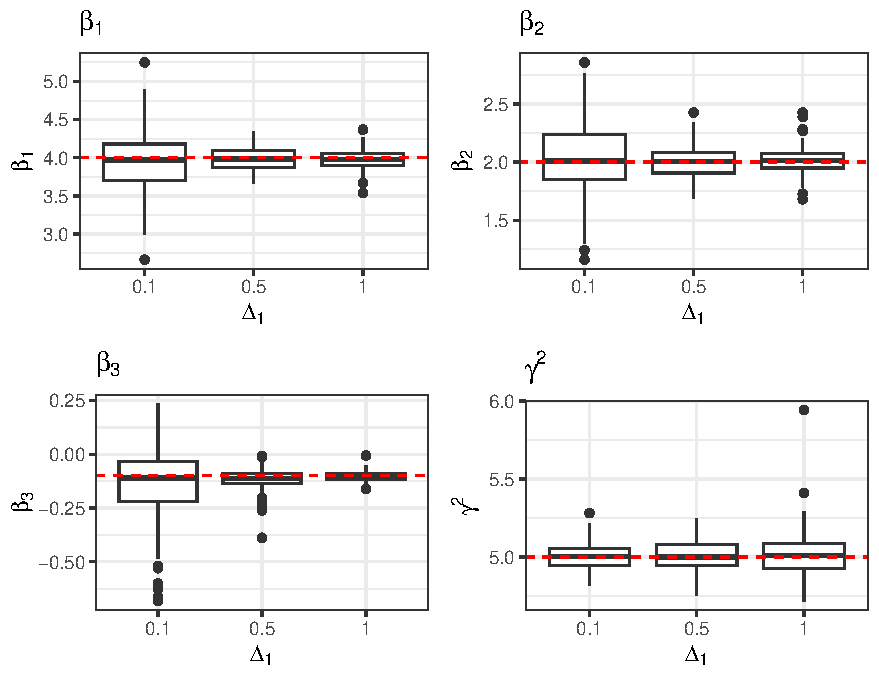
\includegraphics[width=\linewidth]{Images/Results/varying dt plot brownian bridge likelihood.pdf}
    \caption[Box plots of Parameter Estimates for various observation intervals]{box plots showing how the parameter estimates using the importance sampling estimator, with pre-computed Brownian bridges is affected by the time interval between observations. The red dotted lines show the true values of the parameters.}
    \label{fig:}
\end{figure}


\subsection{Varying Number of Bridge-Nodes}



\subsection{Varying Number of Bridges}

\section{Precomputed Brownian Bridge Importance sampling likelihood}
Three studies were performed for the Langevin likelihood approximation using pre-computed Brownian bridge importance sampling. The first by testing the method on tracks with varying time resolutions, the second by testing the method with a varying number nodes in the Brownian bridges and the third by testing the method for a varying number of bridges.

\subsection{Varying time resolution}
To test the method at various resolutions, 100 tracks were simulated from the Langevin process. These tracks were thinned, so that the interval between observation were $\Delta_t \in \{0.1, \ 0.5, \ 1\}$. They were then shortened so each track contained 5000 observations. For each of these 300 tracks, the parameters $\gamma^2$ and $\beta$ were estimated. The result of these estimations are shown in figure~\ref{fig:varying thin boxplot precomputed BB}.

\begin{figure}[H]
    \centering
    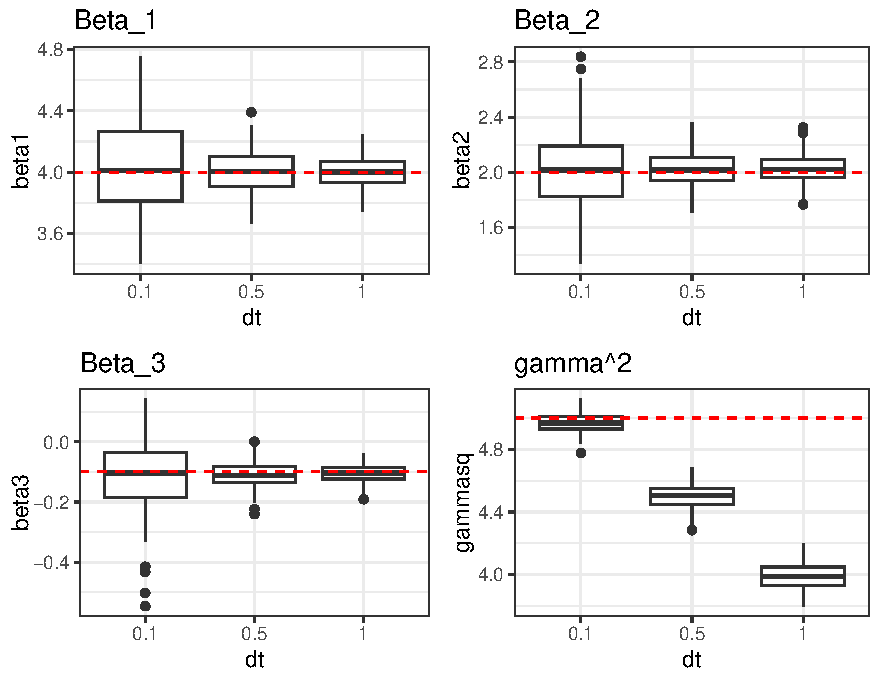
\includegraphics[width=\linewidth]{Images/Results/varying dt estimates precomputed BB.pdf}
    \caption[Box plots of Parameter Estimates for various observation intervals]{box plots showing how the parameter estimates using the importance sampling estimator, with pre-computed Brownian bridges is affected by the time interval between observations. The red dotted lines show the true values of the parameters.}
    \label{fig:varying thin boxplot precomputed BB}
\end{figure}

Figure~\ref{fig:varying thin boxplot precomputed BB} shows that this estimator is an improvement on the \cite{michelot_langevin_2019} for all the parameters. at a thinning of 10 there is little to no bias observed in the estimates based on the simulations, whereas using the \cite{michelot_langevin_2019} there is a noticeable bias at this level of thinning. For the speed parameter $\gamma^2$ figure~\ref{fig:varying thin boxplot precomputed BB}t shows that there is a bias which is observed for thinning of 50 and 100. in both of these cases all the estimations done, significantly underestimated the value of the parameter. One reason for this must be that the Brownian bridges become a much worse proposal density when the speed parameter used for generating the Brownian bridges deviates from the parameter which is being used to compute the likelihood. From figure~\ref{fig:EM_thin_boxplot} we can see that, for a thinning of 10, the estimated speed parameter is around 4.8 when using the same setup as used above. This suggests that the importance sampling likelihood estimate is robust against some deviation in $\gamma^2$ between the simulation of the bridge and the computation of the likelihood based on the bridge. However, as the error increases it leads to a bias in the estimated likelihood.

\

A striking feature of these estimations, is that even though there is a large bias in the speed parameter $\gamma^2$, there appears to be little or no bias in the estimates of $\beta$. This is particularly interesting, since the drift term in the Langevin process is scaled by $\gamma^2$. This might suggest that the variance used in making the Brownian bridges is not that important when it comes to estimating $\beta$, but is more important when it comes to estimating $\gamma^2$.

\ 

\cite{michelot_langevin_2019} observes that when the number of observations used to estimate is held constant, but the distance between the observations increases, the variance of the estimates for $\beta$ decrease. This is also observed in figure~\ref{fig:varying thin boxplot precomputed BB}. \cite{michelot_langevin_2019} attributes this to the fact that the tracks with greater distances explore more of the covariates, and so are less likely to be concentrated on a ...


\

In the simulations done in figure~\ref{fig:varying thin boxplot precomputed BB}, The number of nodes used was the same as the number of nodes used to simulate the Langevin process. We can see how the parameter estimates 



- no visible bias in beta
- variance reduces as distance increases for beta
- bias for gamma
- same variance over time for gamma
- we can compare this to the EM method


\subsection{Varying Number of Bridge-Nodes}
To test the effect of the number of bridge-nodes on the estimates, 100 tracks were simulared from the Langevin process and then thinned so that the interval between observations became $\Delta_t =1$. These tracks were then estimated using the importance sampling likelihood with precomputed Brownian bridges using numbers of bridge nodes $N =\{4,9,49,99\}$. The resulting estimates are displayed as boxplots in figure~\ref{fig: varying N boxplots precomputed brownian bridge}. The code for generating this figure can be found in the GitHub repository under the filename "varying N estimates precomputed Brownian bridges.R".


\begin{figure}[H]
    \centering
    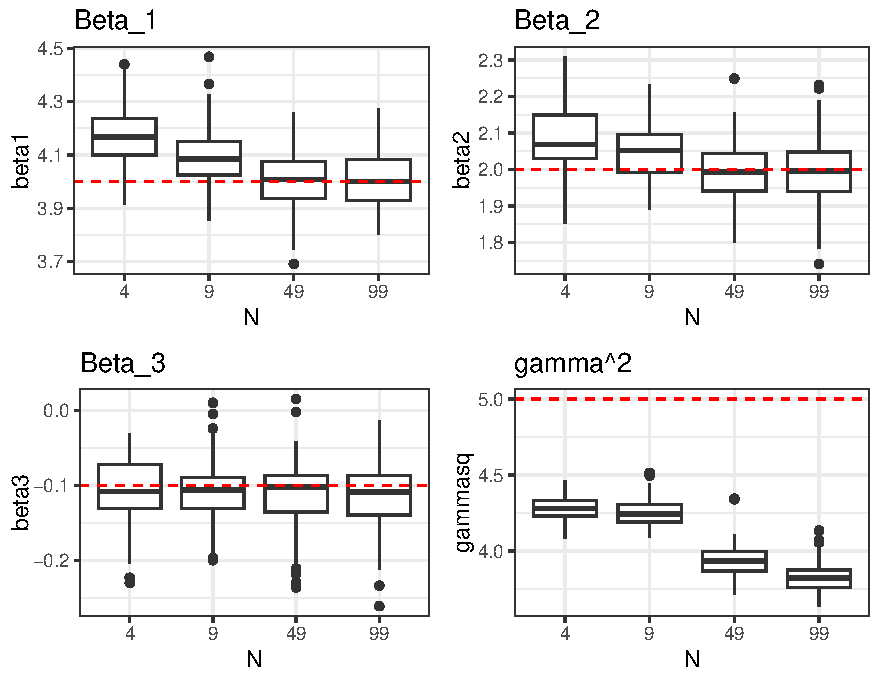
\includegraphics[width=\linewidth]{Images/Results/varying N estimates.pdf}
    \caption[Box plots of Parameter Estimates for various Ns]{box plots showing how the parameter estimates using the importance sampling estimator, with pre-computed Brownian bridges is affected by how many nodes N are used in the Brownian bridges. The red dotted lines show the true values of the parameters.}
    \label{fig: varying N boxplots precomputed brownian bridge}
\end{figure}

Figure~\ref{fig: varying N boxplots precomputed brownian bridge} shows that as the for $N=99$ and $N=49$ there is no observable bias in the estimates for $\beta$.as the number of nodes in the bridges decreases however, there is an increasing bias observed for $\beta_1$ and $\beta_2$. This bias is in the direction away from zero. For $\gamma^2$ there is a bias for all values of $N$ tested, which is consistent with what was experienced for observation interval length of $\Delta_t$ in figure~\ref{fig:varying thin boxplot precomputed BB}. This bias is reduced as the number of bridge-nodes decreases.

\subsection{Varying Number of Bridges}
To study the effect of the number of bridges $M$ on the estimates using the importance sampling likelihood with precomputed Brownian bridges, 100 tracks were simulated from the Langevin process. each track was estimated using importance sampling with precomputed brownian bridges for numbers of bridges $M=\{5,10,50,100,200\}$ and $N=49$ bridge nodes for all these cases. The resulting estimates are displayed as boxplots in figure~\ref{fig:varying M boxplots precomputed brownian bridge}

\begin{figure}[H]
    \centering
    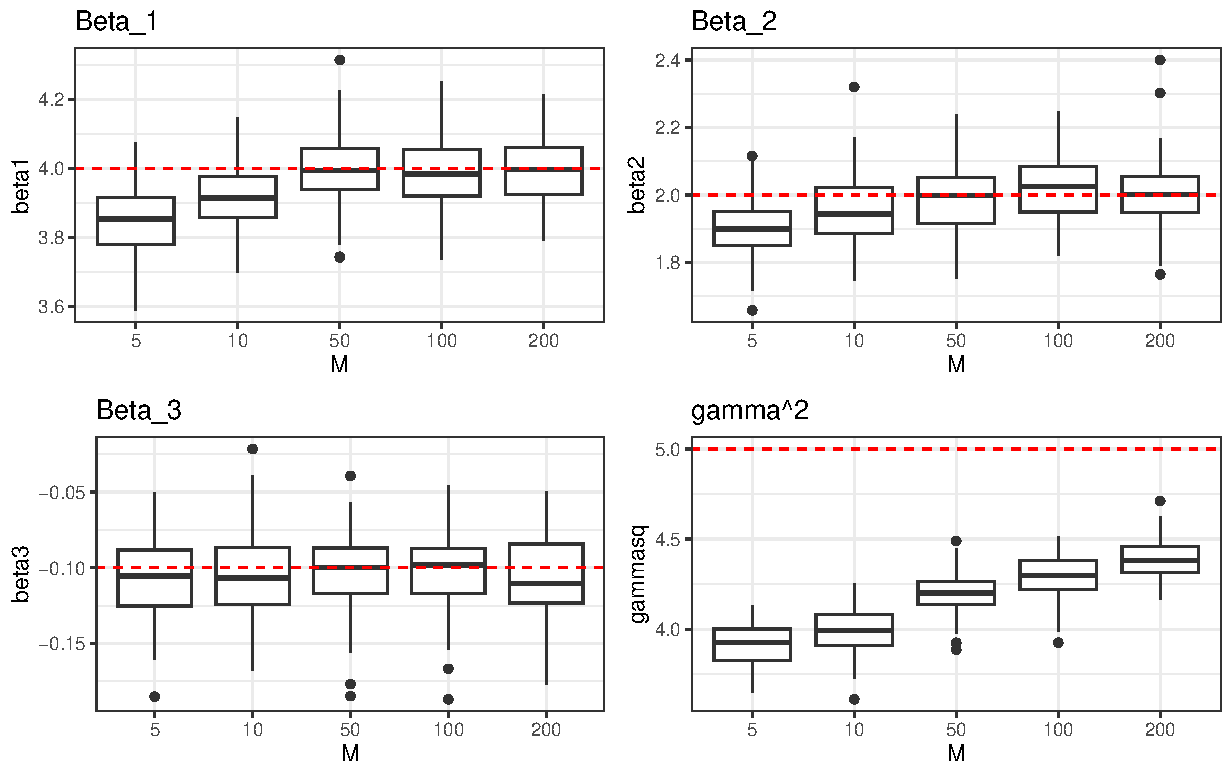
\includegraphics[width=\linewidth]{Images/Results/varying M estimates boxplot precomputed BB.pdf}
    \caption[Box plots of Parameter Estimates for various Ns]{box plots showing how the parameter estimates using the importance sampling estimator, with pre-computed Brownian bridges is affected by how many nodes N are used in the Brownian bridges. The red dotted lines show the true values of the parameters.}
    \label{fig:varying M boxplots precomputed brownian bridge}
\end{figure}

Figure~\ref{fig:varying M boxplots precomputed brownian bridge} shows that there is a large bias in $\beta_1$, $\beta_2$ and $\gamma^2$ when the number of bridges is small. When 